%!TEX root = ../report.tex

\section{Architecture}
\label{sec:architecture}

In this section we first clarify our assumptions about the \emph{application stack} of a SaaS. Then we explain the different architectures to implement  SaaS versioning.

One important assumption we make for versioning is, that each tenant and therefore also all users of a tenant use the same version at the same time. In practice this means that each tenant has a dedicated migration point in time at which they decide to switch the version. This switch affects all their users at the same time. Users aren't allowed to individually choose their version.

We furthermore assume that all requests to the SaaS are authenticated, thus there is always a user as well as a tenant and its version associated with each request.

\subsection{Application stack}
\label{sec:stack}

\begin{wrapfigure}{r}{0.28\textwidth}
  \begin{center}
    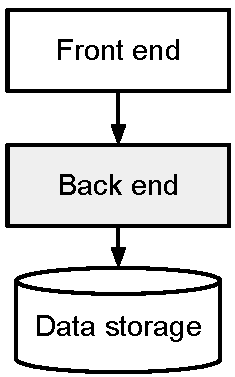
\includegraphics[width=0.28\textwidth]{stack.pdf}
    \caption{Simplified \protect\\ Application Stack}
    \vspace{-20pt}
    \label{fig:stack}
  \end{center}
\end{wrapfigure}


To understand the architecture better, we first want to look at the SaaS application stack as displayed in Figure~\ref{fig:stack}. We derived this stack from our experience with developing SaaS ourselves as well as stacks we have seen in related papers as depicted earlier in Section~\ref{sec:relatedwork}.

We assume a separation between the front end, back end and database layer. The \emph{front end layer} is mainly concerned with the user interface. In a SaaS it will usually be delivered to the user's browser within a HTTP request/response cycle. Another possible implementation for the front end layer is a webservice API that enables external applications (e.g. third-party or native applications) to communicate with the SaaS. We handle this more in-depth in Section~\ref{sec:sharedfrontend}. The \emph{back end layer} is concerned with the application and business logic. It handles requests of the front end layer and consequently communicates with the \emph{database layer}. To allow for horizontal scaling, the front end and back end layers are usually implemented stateless. All state is then kept in the database layer.

To focus our research, we omitted some details of the stack. We were not concerned with neither caching nor load balancing. Furthermore we omitted how user management is done, especially with regards to authentication.

\subsection{Multi-instance}

\begin{figure}
\vspace{-20pt}
\centering
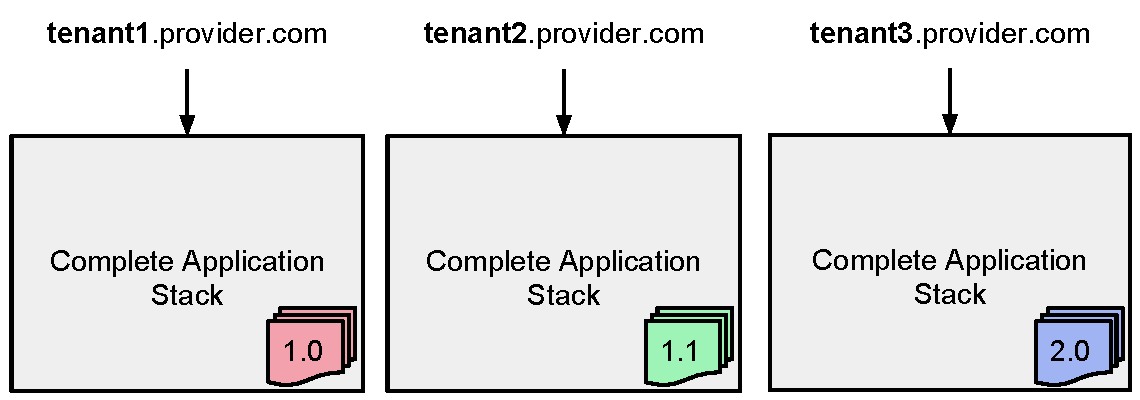
\includegraphics[width=\textwidth]{multiinstance.pdf}
\caption{Example for multi-instance with the respective software version for each tenant deployed on their instance}
\label{fig:multiinstance}
\vspace{-10pt}
\end{figure}

In a multi-instance architecture the whole application stack is deployed several times on dedicated resources. You can see an example in Figure~\ref{fig:multiinstance}. The multi-instance architecture serves the purpose of physical isolation of the tenants by provisioning resources for each tenant individually. Also it allows for developing a single-tenant application instead of building multi-tenancy awareness into the application.

This approach can also be used for versioning, where we see two variants:

\paragraph{Single instance per tenant} When every tenant has their own application stack instance running, these instances can be versioned by deploying the respective software version on the tenant's instance. See Figure~\ref{fig:multiinstance} for reference.
\paragraph{Single instance per version with multiple tenants} This is a hybrid approach where each instance has a specific version and the instances in turn can be hosts for multiple tenants by using the shared-instance mechanisms explained in the following section. See Figure~\ref{fig:multiinstance_versionstack} for reference.

\begin{figure}
\vspace{-15pt}
\centering
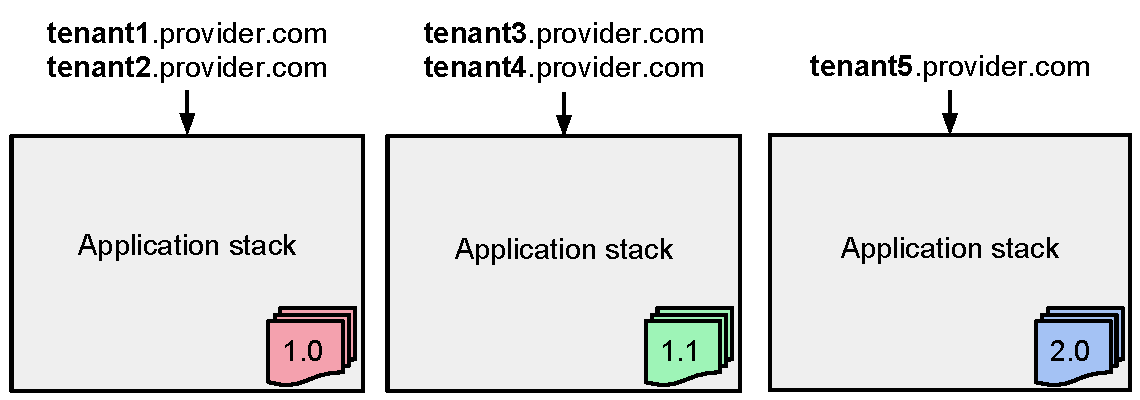
\includegraphics[width=\textwidth]{multiinstance_versionstack.pdf}
\caption{Example for a hybrid multi-instance approach which is multi-instance regarding the version, but shared-instance regarding the tenants}
\label{fig:multiinstance_versionstack}
\end{figure}

Using a multi-instance architecture has the benefits that the developers do not have to deal with issues concerning multi-tenancy in the application code. One of the drawbacks is the bad resource consolidation factor, thus if e.g. one tenant uses many resources but another uses none, the unused resources can't be allocated to the spiking tenant easily. Also the maintenance cost increases with the number of versions and tenants and there is no economy of scale working in favor of the SaaS provider then.

Versioning-wise the actual application stack is not version-aware and thus can be built without versioning as a concern. Instead versioning is handled on the deployment level. Migrations between versions might then need significant operations engineering effort.

\subsection{Shared-instance}

The shared-instance architecture consist of one software stack deployment that serves all tenants at the same time. This architecture is the one that is generally referred to when talking about multi-tenant SaaS applications, since it uses the economy of scale well due to its high consolidation factor \cite{Mietzner2009} \cite{Bezemer2010} \cite{Chong2006}.

To investigate versioning in the shared-instance architecture, we will individually inspect the layers of the application stack as outlined in the previous section, consisting of the front end, back end and database layer. For each layer we will outline how versioning can happen. We are closing this section with a look at how to migrate between versions.

\subsection{Shared-instance: Front-end layer}
\label{sec:sharedfrontend}

We split the \emph{front end layer} into two categories: a \emph{web application} running in the user's browser and an \emph{API consumer} e.g. running on the user's mobile phone.

\subsubsection{Web application} In web applications the user's browser is usually reloading the whole web page on each request, which mostly is triggered by an interaction of the user with the system\footnote{We assume that caching works transparently and perfectly as well as "One page applications" reloading their assets automatically ("hot code reload") in case something on the back end layer changes, as explained in \url{http://www.meteor.com/blog/2012/02/09/hot-code-pushes}}. Thus there is a tight coupling between the front end and the back end layer, from which we conclude that they are both versioned simultaneously. Since the front end software is delivered to the user's browser on each request, the versioning concern can be completely handled on the \emph{back end layer} as outlined in the next section.

\subsubsection{API consumer} To allow programmatic access to the SaaS functionality, SaaS providers usually implement a webservice. A common occurrence are HTTP APIs following the REST principles \cite{Fielding2000}. These APIs allow native applications (e.g. mobile phone applications) or other webservices to build on top of the SaaS. The SaaS and their API consumers are loosely coupled. They follow their own product cycles. In case of compatibility breaking changes in the SaaS API, the API consumers have to adapt to the changes and deploy a new version to their users. This might be hard to do e.g. because users might be reluctant to updates, delivery cycles might be too long or the API consumer developer might not have the resources to update their product. This leads us to the conclusion that SaaS APIs should be able to provide several versions at the same time. The API consumers choose which version of the API they want to use. There are many ways to handle versioning APIs and explaining them in-depth is out of the scope of this report. Examples are version numbers in the URL or \emph{HTTP Accept Header} of a request \cite{RFC2616}, or feature flags for the consumer application in the SaaS \cite{playbook2013} (as explained further in Section~\ref{sec:shared1n}).

  % Frontend API Versioning
  %   In URL:
  %     http://api.com/v1/resource.json?version=1
  %   Accept Header:
  %     Accept: application/json+v1
  %   Application Flag:

\subsection{Shared-instance: Back-end layer}
\label{sec:backend}

For versioning the back end layer we explore two variants: \emph{1:1} and \emph{1:n}.

\subsubsection{Shared-instance with 1:1 mapping}

\begin{figure}[h!]
\centering
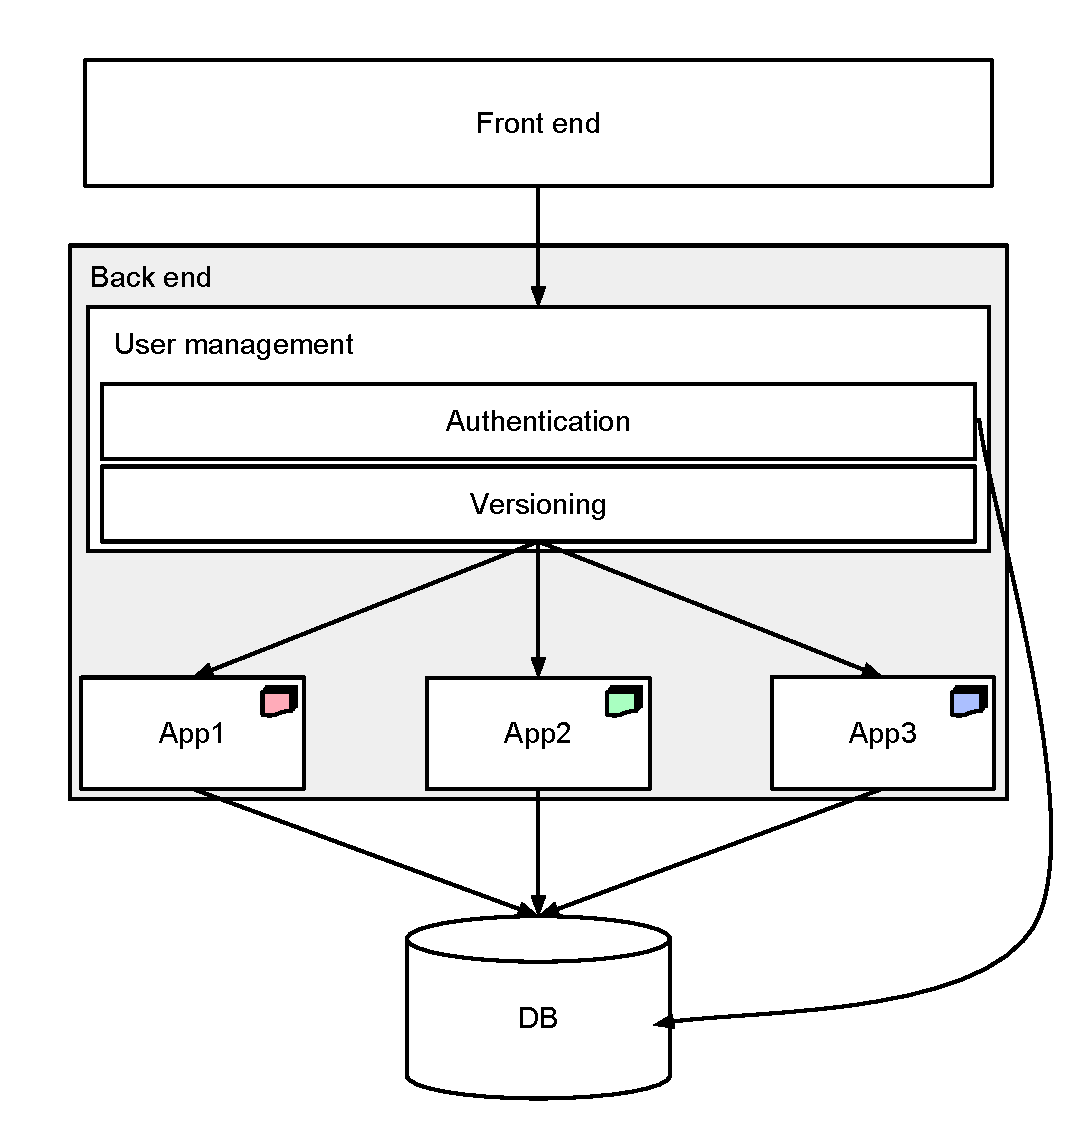
\includegraphics[width=\textwidth]{sharedinstance11.pdf}
\caption{Example for a shared-instance architecture with mapping each back end server to a code revision which in turn 1:1 maps to a product version}
\label{fig:sharedinstance11}
\end{figure}

The \emph{1:1 mapping} depicts that each product version is mapped to one code revision. Figure~\ref{fig:sharedinstance11} shows the architecture. Thus to support different product versions at the same time, the respective code revisions have to be deployed on different back end servers. On each request, the user management decides to which back end servers the request is routed, depending on the tenant the user belongs to.

The benefit of this approach is, that the versioning is happening outside of the application code, thus the code does not have to be version-aware. On the downsides, the consolidation factor of this approach is low, given that the load is split between non-consolidateable versions. This defecit increases with the increase of versions running in parallel. Furthermore this leads to a heterogeneous deployment which is more complex than a homogeneous deployment.  Also this can lead to problems like bugfixes, that if written once have to be merged and deployed into every running version. Also this approach needs an intelligent routing layer (in our example above the user management) which decides on which app server to map which request.

% a product ver = code rev
%
% Pro
% Versioning is external to application code
%
% Contra
% worse consolidation factor
% intelligent routing layer needed
% heterogeneous deployment
% forking of code base makes security patches difficult to apply

\subsubsection{Shared-instance with 1:n mapping}
\label{sec:shared1n}

\begin{figure}
\centering
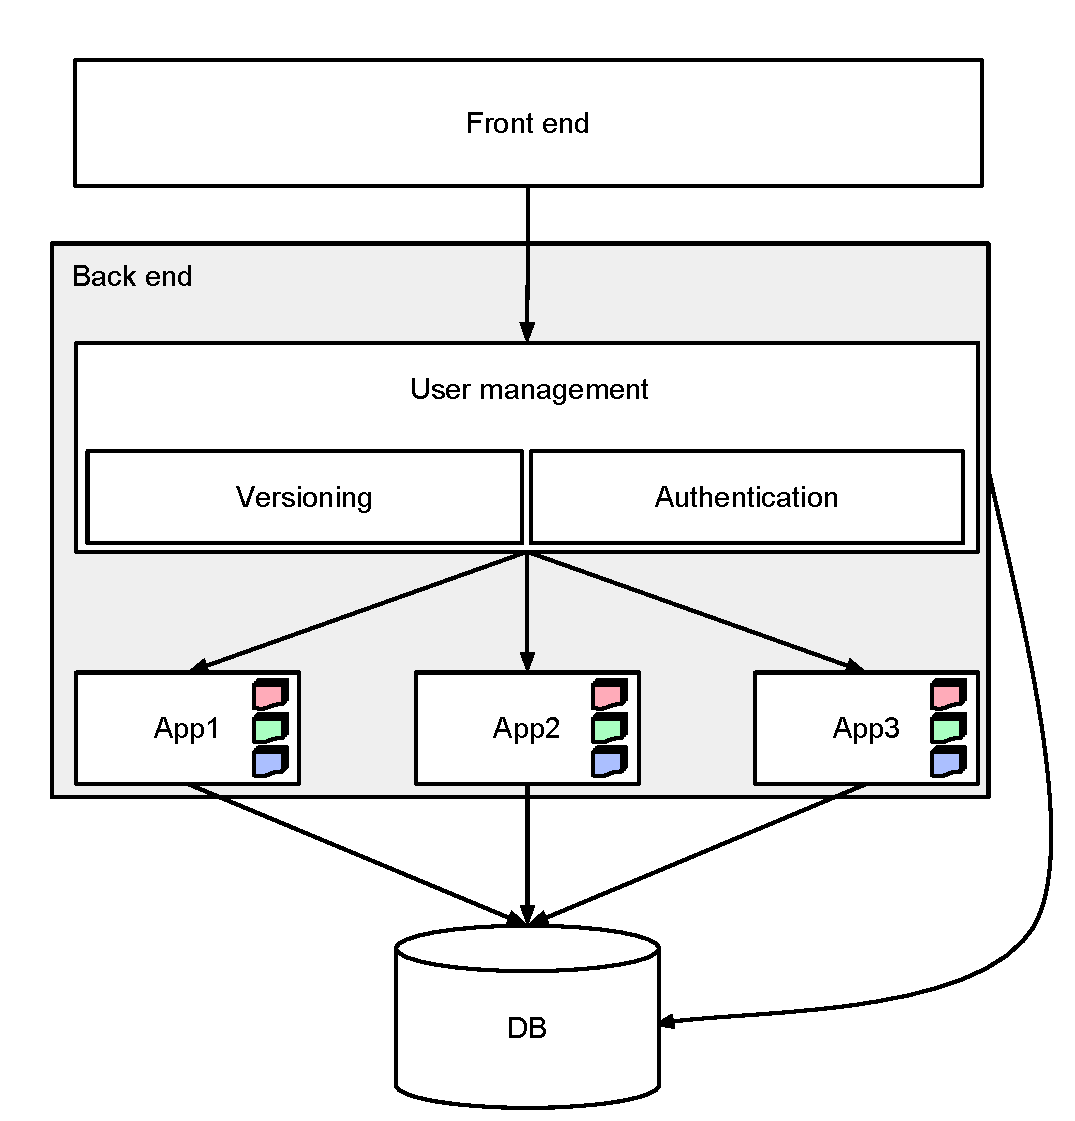
\includegraphics[width=\textwidth]{sharedinstance1n.pdf}
\caption{Example for a shared-instance architecture with 1:n mapping}
\label{fig:sharedinstance1n}
\end{figure}

The \emph{1:n mapping} depicts that each code revision maps to all available \emph{n} product versions. As shown in Figure~\ref{fig:sharedinstance1n} each application server has the same code revision deployed and is therefore able to decide which product version to serve for each request. One way to implemented this is with feature flags. Listing~\ref{1ncode} shows a code example in Ruby. In the beginning of this section we assumed that every request has a user attached to it. Furthermore we assumed that all users of a tenant share the same version. This leads us to the conclusion, that the backend can determine the version for each incoming request.

\noindent\begin{minipage}{\textwidth}
  \lstset{language=Ruby, caption=Example code for \emph{1:n mapping} on an application server, label=1ncode}
  \begin{lstlisting}
    if user.has_version?("1.0")
      do_something()
    end

    if user.has_version?("1.1")
      do_something_a_bit_different()
    end
  \end{lstlisting}
\end{minipage}

The \emph{1:n mapping} approach has several benefits: The consolidation factor is high, since all app servers can serve all requests. The deployment is homogeneous over the app servers, thus making operations easier. Also it is possible to version more fine-grained, not only based on product versions but actually on feature level and even feature version. This opens up a tenant-feature matrix which allows versioning which is more flexible than the traditional linear versioning.
On the downside, the feature flags in the code increase code complexity, which might increase development time and increases the probability of bugs. Also the feature flags are spread over the code and removing them needs software development effort. Thus abandoning old versions is connected with extra cost.

% Pro
% good consolidation
% homogenous deployment
% more flexibility: fine grained feature selection
%
% Contra
% increased code complexity, might lead to more bugs
% high cost for abandoning old version to clean code base
%
%
% inside of code base are many version checks "if version == 1.4 ..."
% more flexibility in choosing version, maybe not choose version but choose only features

\subsection{Shared-instance: Database}
\label{sec:database}

The database is where state is kept. We assume that the database is in the style of a relational database, in that it keeps the data in tables with specified schemas to ensure the format and validitiy of the data.

In this section we will differentiate between two major cases reagarding the database when versioning SaaS: \emph{Different versions share the same datbase schema} and \emph{different versions need separate schemas}.

\subsubsection{Different versions share a compatible schema}
% TODO nice diagram?

When different versions share the same database schema, the database is actually agnostic to versioning. The changes of the versions happen in the other layers and thus never propagate down to the database. The same happens if changes are needed for one version, but the changes are compatible with the other versions. An example for this is the addition of new columns or tables. These can usually be ignored by versions that don't need these columns or tables, thus enabling compatiblity with the changed schema.

\subsubsection{Different versions need incompatible schemas}
% TODO nice diagram?

When schemas change between versions in an incompatible way, the database shares the concern of versioning. Given that we assume we are dealing with a schema-based database management systems, the question is: How can database schemas be versioned? How can a database support several schemas for the same data at the same time?

In our research we did not find a database that prodvides version-aware schemas. We investigate this option more in Section~\ref{sec:futurework}.

% TODO materialized views? i remember some research about making them writeable as well ...

Since the database can not handle the versioning concern, the responsibility is pushed up in the stack to the back end layer again. Next we will investigate two approaches for that.

\paragraph{Different tables for each schema}

To store different schemas, a new database or table can be created for each version. An example with different tables can be seen in Listing~\ref{differenttablessql}. Each tenant is on a specific version, thus their data is stored in the table for their respective version.

\lstset{language=SQL, caption=sql, label=differenttablessql}
\begin{lstlisting}
  create table users_v1;
  create table users_v2;
  create table users_v3;
\end{lstlisting}

% TODO: Ich bin von den Pro/Cons nicht so richtig überzeugt
% Pro:
% Works well if not too many versions
%
% Con:
% Messy design if many versions

\paragraph{Pivot tables}

\begin{figure}
\centering
\includegraphics[width=\textwidth]{pivot.png}
\caption{Schema of pivot tables as shown in \cite{Yaish2011}}
\label{fig:pivot}
\end{figure}

Pivot tables as explained in \cite{Yaish2011} \cite{Aulbach2011} \cite{Weissman2009} follow the idea of not using a fixed schema in the database but keeping a flexible schema in the application. The database gets reduced to a more simple key-value store. An example can be seen in Figure~\ref{fig:pivot}.

\subsubsection{Migration of data}

When a tenant decides that they want to move to a new version and the version switch changes the schema, then the data of the tenant has to be migrated from the old to the new schema. Next we will describe two ways for running migrations:

\paragraph{Batch-processing migration} The data is migrated in one go. Depending on the database management system, the schema changes and the amount of data, this process might take significant time. Depending on the algorithm used to execute the migration, the database might be completely unavailable for that tenant's users during the migration or be in a read-only state.

\paragraph{On-the-fly migration} The data is migrated when it is requested or written. This could mean that clusters of data are migrated in batch (e.g. a user is migrated when she logs in) or are migrated row-by-row.

% version is chosen per tenant
% data migrations need time
% data migrations might need downtime
% on-the-fly migrations possible
